% TEMPLATE for Usenix papers, specifically to meet requirements of
%  USENIX '05
% originally a template for producing IEEE-format articles using LaTeX.
%   written by Matthew Ward, CS Department, Worcester Polytechnic Institute.
% adapted by David Beazley for his excellent SWIG paper in Proceedings,
%   Tcl 96
% turned into a smartass generic template by De Clarke, with thanks to
%   both the above pioneers
% use at your own risk.  Complaints to /dev/null.
% make it two column with no page numbering, default is 10 point

% Munged by Fred Douglis <douglis@research.att.com> 10/97 to separate
% the .sty file from the LaTeX source template, so that people can
% more easily include the .sty file into an existing document.  Also
% changed to more closely follow the style guidelines as represented
% by the Word sample file. 

% Note that since 2010, USENIX does not require endnotes. If you want
% foot of page notes, don't include the endnotes package in the 
% usepackage command, below.

% This version uses the latex2e styles, not the very ancient 2.09 stuff.
\documentclass[letterpaper,twocolumn,10pt]{article}
\usepackage{usenix,epsfig,endnotes,color}
\usepackage{multicol}
\usepackage{parcolumns}
\usepackage{lipsum}
\usepackage{paracol}
\usepackage{graphicx}
\usepackage{float}
\usepackage{hyperref}
\usepackage{booktabs}
\usepackage{amsmath}
\usepackage[linesnumbered,ruled]{algorithm2e}



\begin{document}

%don't want date printed
%\date{}

{%
%\begin{center}
%{\large \bf CS 516 Paper Review Title}
%\end{center}


%\begin{center}
%Your Name
%\end{center}

%alternate box header
\noindent \fbox{
\parbox{0.45\textwidth}{
{\bf \large CS 415/516 Assignment 3}
\par
{\bf \large Title: Parallelizing Markov Decision \\Process Problems}
\par
{\bf \large Name: Arthur Quintanilla and \\ Ankith Kolisetti}
}
}

\section{Introduction}

Markov Decision Process (MDP) problems are used in a subset of machine learning known as reinforcement learning. They have been used in a wide variety of applications such as optimizing profit through supply and demand (how much to produce given demand) [1], optimizing stock investments [1], and in one case it has also been used to have a machine intelligently recognize the identity of a speaker by their voice [2]. 

For our research we consider MDP problems and the Value Iteration algorithm that is used to solve them. We consider the sequential version of this algorithm and seek to exploit within it areas that would lend themselves to parallelization. The lack of dependency between states to update utility values, and the use of a previous and current buffer are particularly lucrative in this regard.

We also considered the sequential Value Iteration algorithm and used this as a standard to test the correctness of our parallelized version. The evaluations include different block size and block number configurations, different map sizes, and larger reward sizes. Each of these factors was considered and will be compared to the run-time of the sequential algorithm.


\section{Background}

To simulate real-world utilities for our research project, we created a test file data generator that would randomize $n\times m$ grid worlds in which the agent could perform any of four actions at each time-step. Since we are simulating a grid world, we called these actions up, down, left, and right which are represented by integer values in our code.

In MDP problems, actions are non deterministic. We simulate this in our grid world by establishing that the agent succeeds in its chosen action 80\% of the time. 10\% of the time the agent will instead move in the direction $90^\circ$ counter-clockwise (so if it wanted to go up it would instead go left) and the final 10\% of the time it would instead move in the direction $90^\circ$ clockwise. If the agent tries to move out of the bounds of our grid world, this action always fails.

In order to simplify our transition model we say that the only possible transitions an agent can make from state $s$ to $s^\prime$ is either $s$ itself (no transition) or to an $s^\prime$ directly adjacent to $s$. The action that the agent takes to potentially achieve this transition is denoted as $a$ and the probability of this transition occurring is denoted as $p$. Then, we can define our transition model as $T(s,a,s^\prime)=p$.

Here is a small snippet of one of our sample transition models that we use to test our code.

\begin{center}
	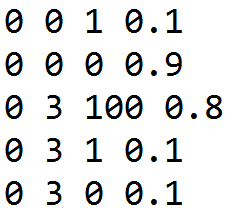
\includegraphics[scale=1.0]{tmodel_snippet}
\end{center}

This is a list of the transitions for state 0 when the agent takes action 0 or 3. According to this transition model, when the agent takes action 0 at state 0, it will stay at state 0 with probability 0.9 and move to state 1 with probability 0.1. Similarly, if the agent takes action 3 at state 0, it will move to state 100 with 0.8 probability, move to state 1 with 0.1 probability, and stay at state 0 with 0.1 probability. 

In the sequential algorithm, each of these individual entries in the transition model must be iterated over for \textit{one} iteration of the algorithm. Depending on the convergence criteria this this implies the algorithm can take a very long time to reach a solution. In the $100 \times 100$ grid world that we did most of our testing on there were 119,992 total transitions. Since there is no dependency between states, these are perfect conditions for parallelization.

In our parallel implementation we will assign each entry in the transition model its own thread. The summation step can be quickly computed by using $atomicAdd$ operations to accumulate the summation for each action in each state in a temporary buffer. After all of these have been computed we select for each state the action with the maximum utility, multiply this by the discount factor, and add it to the reward value of $s$ to get the updated utility for $s$. The entire formula is seen below.

\begin{center}
	$U^\prime(s)=R(s)+\gamma * max_\alpha \sum_{s^\prime}T(s,\alpha,s^\prime)*U(s^\prime)$
\end{center}

Note how we update $U'$ at each iteration using $U$ from the previous. Thus we can use out of core buffer swapping manage these arrays.

Also, we define $R(s)$ as the reward of state $s$. The reward is some benefit or harm that the agent receives for existing at $s$ represented by a positive or negative value. For our purposes we consider positive values to be desirable and negative values undesirable.

The discount factor $\gamma$ "discounts" actions that occur further down the line. In concept this means we can predict our utility better a few moves ahead rather than many moves in advance, and so earlier actions should be weighted more heavily according to the discount factor.

At each iteration, applying this formula will propagate utility values in such a way that immediate rewards become negligible compared to the possible rewards in the future. This supplies our agent with the ability to know the best choice of action for each state it finds itself in. This has many useful applications in the area of machine learning.

\section{Implementation Details}

There are two main steps to each iteration of the sequential algorithm. The first step is to calculate for each action at each state the utility that that action can provide to the agent at the current time-step. This is calculated by taking the summation of all $T(s,\alpha,s^\prime)$ for each action at each state. 

Essentially we first partition the transitions by state. Then we partition those partitions by actions. We take the summation of the transition probability multiplied by the current utility of $s^\prime$ for that transition, and sum it into a buffer for the corresponding state and action.

The first step must complete in its entirety before the second step can begin, as it is dependent on the intermediate utility values calculated there. Since the $\_\_syncthreads$ call only synchronizes threads across a similar block, we found the most practical way to approach this synchronization challenge was to implement one iteration of the algorithm using two kernel calls, one for the action summation step, and the other for the utility update step.

The utility update step includes determining the action that yielded the highest utility to a state at the current time step. We then take this maximum utility value and multiply it by the discount factor and add that value to $R(s)$. This gives us our updated $U^\prime(s)$ value for the current iteration.

We were unable to properly implement a parallel reduce $\_\_device\_\_$ function within the time constraints required for this research project, so we implemented the maximum finding sequentially and did the computation step in parallel. However, utilizing parallel reduction here to find the maximum action utility value for each state would certainly be a great exercise in optimization.

\scriptsize 
Note that the following benchmarks were done using a thread block specification of 1024 blocks and 1024 block size.
\normalsize

\subsection{Action Utility Summation}

This part of the algorithm was the part that we found parallelism was best exploited. This makes natural sense as the transition model is the largest structure in this algorithm that must be iterated over at each step. Since we are representing our simulated grid world through this transition model it can essentially be thought of as a directed graph. Each edge of the graph is then an entry in the transition model. Typically in MDP problems there are many edges between states, so this is a great point at which to exploit the parallelism available.

%Below is the pseudo-code for our parallel implementation of the action utility summation:
%
%\begin{algorithm}
%	\SetKwInOut{Input}{Input}
%	\SetKwInOut{Output}{Output}
%	
%	\underline{function Euclid} $(a,b)$\;
%	\Input{Two nonnegative integers $a$ and $b$}
%	\Output{$\gcd(a,b)$}
%	\eIf{$b=0$}
%	{
%		return $a$\;
%	}
%	{
%		return Euclid$(b,a\mod b)$\;
%	}
%	\caption{Action Utility Step - Parallel Implementation}
%\%end{algorithm}

Let $ns$ be the number of states and $na$ be the number of actions specified in the MDP. At this step in the algorithm we will have an array of size $ns * na$. This is because for each state we need to have a separate element for each action to accumulate the results of the summation into. Since the read-modify-write operations must take place in order we will use $atomicAdd$ to compute the summation. Below is a table representing the speedup we saw in this step in our parallel implementation as compared with the sequential algorithm.

\begin{table}[h!]
	\centering
	\caption{Action Utility Summation Times}
	\label{tab:table1}
	\begin{tabular}{ccc}
		\toprule
		Benchmark & Sequential & Parallel\\
		\midrule
		Sample1 & 0.289ms & 1.715ms\\
		Sample2 & 1.135ms & 2.518ms\\
		Sample3 & 7.194ms & 8.613ms\\
		\bottomrule
	\end{tabular}
\end{table}

\scriptsize
Note that these times are for one execution of this step, not across the entire algorithm
\normalsize

\begin{itemize}
	\item Sample1 is a $100\times100$ grid world with 119,992 transitions.
	\item Sample2 is a $200\times200$ grid world with 479,992 transitions.
	\item Sample3 is a $500\times500$ grid world with 2,999,992 transitions.
	\item Sample4 is a $750\times750$ grid world with 6,749,992 transitions.
\end{itemize}

As the results seem to suggest, no matter how large we made the number of transitions in the transition model, the parallel implementation was always $\sim$1.5ms slower than the sequential implementation. We believe this has to do with the overhead involved in launching the kernel to perform the action utilities summation step however we did not implement a way to test this.

One possible way that could be implemented to optimize this step is to re-arrange the way we access the action\_util array to avoid bank conflicts, as this array is not accessed by thread id but rather by the state/action the current thread is processing.

\subsection{Update Utility}

The next step of the parallel implementation is to update the utility values stored in $U^\prime$ using the maximum action utility of each state that we calculated in the previous step of this same iteration. In the sequential algorithm, this step is dependent on each state. Each state must query every possible action it can take, decide which action has the greatest utility, and select that utility value to update its $U^\prime(s)$ value. However, there is no inter-dependency between the states themselves, which means each state can update its utility value independent of every other state. Again, this leaves a lot of room in the algorithm to find areas for parallelization.

One thing that is important to note is that it is absolutely imperative before this step begins that all of the action utility values from the previous state must have already been computed. Once we have these values, for each state we will select the utility of the action that yielded the largest utility value. We multiply this value by the discount factor and add it to the reward $R(s)$ value. This is the state that is called Update Utility.

We implemented this step by assigning each thread to process a single state. The thread will look at each utility value for each possible action the agent can perform at that state and select that maximum one. This is the value that will then be used to update the $U^\prime(s)$ in accordance with the formula.

Unfortunately we were not able to implement a parallel reduction $\_\_device\_\_$ function before we reached the time limit for this project. But it is perhaps another area for optimization that we could work on in the future. Because we did not have this working on time, we searched for the maximum utility for each state sequentially, and then proceeded to do the update formula in parallel.

We achieved the following comparative results:

\begin{table}[h!]
	\centering
	\caption{Utility Update Times}
	\label{tab:table1}
	\begin{tabular}{ccc}
		\toprule
		Benchmark & Sequential & Parallel\\
		\midrule
		Sample1 & 0.146ms & 1.276ms\\
		Sample2 & 0.635ms & 1.352ms\\
		Sample3 & 3.507ms & 1.836ms\\
		Sample4 & 8.017ms & 2.613ms\\
		\bottomrule
	\end{tabular}
\end{table}

\begin{itemize}
	\item Sample1 is a $100\times100$ grid world with 10,000 states.
	\item Sample2 is a $200\times200$ grid world with 40,000 states.
	\item Sample3 is a $500\times500$ grid world with 250,000 states.
	\item Sample4 is a $750\times750$ grid world with 562,500 states.
\end{itemize}

It is important to note that the threads are now assigned states, rather than transitions, so this changes the degree of parallelism achieved from the last step as well as the work being done.

Unlike the previous step however we see that the sequential algorithm does not scale nicely with very large states, whereas the parallel algorithm does not increase in time all that much as the number of states increases by nearly $50\times$. We believe this step scaled much better than the first step because there was no need for atomic operations here. We needed an $atomicAdd$ in the previous step in order to compute the summation. Here, however, since it is just a simple calculation, no atomics are needed, and thus the algorithm enjoys a much better performance in its parallel implementation.

\subsection{Buffer Swapping}

In a similar manner to our SSSP implementation, where we used a dist\_prev and a dist\_curr buffer to store the distance for each node, here we use two buffers to store previous and current utility values for each state. Because of the fact that in on iteration of the algorithm no $U^\prime(s)$ value is dependent on any other $U^\prime(s)$ in the same iteration, we can separate the buffers and use out of core buffer swapping once the kernel calls are complete.

Another area for improvement/future work here would be to see if there is a way to implement in-core buffer swapping to update the $U$ array. However, we were not able to find a way to implement this due to the fact that updating $U$ mid-iteration changes the utility values that other states need to be able to calculate their own, thus changing the desired operation of the algorithm.

\subsection{Convergence Criteria}

It is up to the user to specify the convergence criteria for this algorithm. For all of our benchmarks we chose an epsilon value of $0.001$. Using a discount factor of $0.8$ seemed to be a good balance of fast convergence and accurate results.

\section{Evaluation Results}

For each test we performed the algorithm was able to achieve proper correctness. To visualize the intended function of this algorithm we supply four heatmaps (all generated using a block size of 1024 and a block number of 1024) that display the distribution of the utility values across the simulated grid world. 

\end{document}







